\documentclass[paper=a4, fontsize=11pt,twoside]{article}
% -------------------------------------------------------------------- 
% General Page Layout
% --------------------------------------------------------------------
\usepackage[a4paper]{geometry} 
\usepackage[parfill]{parskip}
\setlength{\oddsidemargin}{5mm}  % Remove 'twosided' indentation
\setlength{\evensidemargin}{5mm}
% --------------------------------------------------------------------
% Encoding and Language Settings
% --------------------------------------------------------------------
\usepackage[T1]{fontenc} 
\usepackage[utf8]{inputenc}   
% encoding may need to be changed depending on the system
\usepackage[swedish]{babel} 
\usepackage{lipsum} % Lorem Ipsum
% --------------------------------------------------------------------
%  Utilities (colors, links, pictures, ect...)
% --------------------------------------------------------------------
\usepackage{xcolor}
\usepackage{hyperref}
\usepackage{graphicx}
\usepackage{amssymb}
\usepackage{epstopdf}
\usepackage[round]{natbib}
\usepackage{float}
\usepackage{placeins}
\usepackage{listings}
\lstset{language=SQL} 
\DeclareGraphicsRule{.tif}{png}{.png}{`convert #1 `dirname #1`/`basename #1 .tif`.png}
% -----------------------------------------------------------------------------%
% Title Page / Document Class Definitions (Please Don't Play With This)
% -----------------------------------------------------------------------------%	
% Table of contents depth = section & subsection
\setcounter{tocdepth}{2}
																								
% Horizontal rule
\newcommand{\HRule}[1]{\rule{\linewidth}{#1}}   														
% Document Number
\newcommand{\documentNumber}[1]{\centering PUSP1742#1 \\[1.0cm]}
				
% Document Version
\newcommand{\documentVersion}[1]{\centering \small{v.#1} \\[1.0cm]}

% Group Responsible
\newcommand{\documentResponsible}[1]{\centering  Ansvarig Grupp: #1}

% Document Creator Group
\newcommand{\documentCreator}[1]{\centering Uppgjord Av: #1}																					
% Title
\makeatletter \def\printtitle{ {\centering \@title\par}} \makeatother
	
% Author .. not really used, but it can stay in case
\makeatletter \def\printauthor{ {\centering \large \@author}} \makeatother

\newcommand{\grouptitlepage}[5]{ 
	\title{
		\documentNumber{#1}																		
		\documentVersion{#2}																			
		\HRule{0.5pt} \\ % Upper rule 
		\LARGE \textbf{\uppercase{#3}} \\
		\large \textbf{\uppercase{ETSF20 Grupp 2}} 
		\HRule{2pt} \\ [1.5cm]    
		\normalsize            
		\documentResponsible{#4} \\ 
		\documentCreator{#5}  
	}																							
	\maketitle																					
	\thispagestyle{empty} 																		
	\newpage 
}
% \grouptitlepage{doc number}{Version Number}{doc title}{group responsible for
% doc}
% --------------------------------------------------------------------------------%
% Title Page / Document Class Definitions (Please Don't Play With This)
% --------------------------------------------------------------------------------%

% \date{}                                            
% Activate to display a given date or keep commented for current date

% -------------------------------------------------------
% DOCUMENT START (YOU CAN IGNORE EVERYTHING ABOVE HERE)
% -------------------------------------------------------
\begin{document}

% -------------------------------------------------------
% Title Page START
% -------------------------------------------------------
\grouptitlepage
% the \# typesets a # character into the document, you will need to replace them
% in yourdocuments. This is a template, just plug in what you need between the
% {}s. Document Code Number (same as time reports)
{14}
% Document Version Number
{0.1}
% Document Title
{STLDD}
% Group Responsible For Document
{(SG)Systemgrupp}
%Document responsible
{(UG)Utvecklingsgrupp}
% -------------------------------------------------------
% Title Page END
% -------------------------------------------------------
\tableofcontents
% WRITE THINGS BELOW HERE

\section{Introduktion}
Detta dokument beskriver högnivådesignen för ett tidrapporteringssystem, E-Kyss. Systemet i fråga är en utveckling utav ett redan befintligt system, ''BaseBlockSystem''. Systemet innehåller flera olika funktioner såsom att skapa tidsrapporter, hålla reda på rapporterad tid utav mindre grupper i projektgruppen. Projektledare har även möjlighet att se en sammanställning utav all rapporterad tid. 

\section{Referensdokument}
\begin{itemize}
\item SRS PUSP174212 version: 0.2
\item BaseBlockSystem STLDD: PUSS1204 version: 1.0 gäller för alla punkter om det inte är specificerat i respektive underrubrik att det som står i PUSS412004 version: 1.0 utgår för specifik del.
\end{itemize}
\section{Terminologi}

\newpage
\section{Översikt}
Systemet är utvecklad för applikationsservern Apache Tomcat, där Java Servlet, JavaServer Pages (JSP) samt Java Expression Language (JSP EL)-teknologier tillämpas enligt JavaEE:s 2:a MVC-modellarkitektur. Systemets huvudfunktion är att fungera som ett tidrapporteringssystem.


\subsection{Vynivå: JSP (JavaServer Pages)}
Nedan förklaras vad varje fil för JSP:n har för betydelse.
\subsubsection{login.jsp}
Denna fil innehåller vy-design som representerar inloggningsformuläret på förgrunds nivå, d.v.s. för den webbsida som är 		publikt tillgänglig utan inloggning. Denna webbsida används för att komma åt bakgrundsnivån för tidrapporteringsapplikationen. Designen består utav en inloggningsfält för användarnamn, ett för lösenord samt en rullista över val av projektgrupper. Kontrollen för denna vy är \textbf{class LoginServlet}.

\subsubsection{groupmanagement.jsp}
Filen innehåller vy-design som representerar projektgrupphanteringen för webbapplikationen som används av administratören. Här finns ett formulärfält för att lägga till en ny projektgrupp, samt en lista över vilka projektgrupper som existerar  i systemet. I denna listan finns funktionen att ta bort aktuell projektgrupp från systemet. Kontrollen för denna vy är \textbf{class GroupManagementSevlet}.

\subsubsection{usermanagement.jsp}
Vy-designen för användarhantering representeras av denna fil. Vyn används av administratör och projektledare där vyn anpassas utifrån användarens behörigheter utifrån dess roll i systemet. Kontrollen för denna vy är \textbf{class UserManagementServlet}.

\subsubsection{reportmanagement.jsp}
Filen innehåller vy-designen som representerar hantering av veckorapporter. Endast projektledaren har tillgång till denna webbsida. Kontrollen för denna vy är \textbf{class ReportManagementServlet}.

\subsubsection{report.jsp}
Filen innehåller vy-designen som representerar skapandet av veckorapporter. Projektledare och användare kommer använda denna webbsida för veckorapportering. Automatiserad signering av projektledarens veckorapportering sker på modellnivå när veckorapporten skickas in till servern. Kontrollen för denna vy är \textbf{class ReportServlet}.

\subsubsection{dashboard.jsp}	
Vy-design som representerar sammanställning av tidrapporter som renderas ut på sidan. I denna vy väljs även hur sammanställningen ska presenteras genom att välja olika renderingsformer av sammanställningen. Kontrollen för denna vy är \textbf{class DashBoardServlet}.

\subsubsection{user.jsp}	
I denna vy-design ser användaren sin personliga information, och kan ändra sitt lösenord. Kontrollen för denna vy är \textbf{ class UserServlet}.

\subsection{Kontrollernivå: Servlet}
Klasserna som specificeras nedan agerar som kontroller i systemet.

\subsubsection{LoginServlet}
Denna kontrollern tar hand om kommunikationen mellan \textbf{login.jsp} och modellen \textbf{LoginBean}, som innehåller information om en given projektgrupp. Denna \textbf{LoginBean} skickas som en lista till \textbf{login.jsp} för att rendera ut valen av projektgrupp vid inloggning.\newline
\newline
\textit{URL-pattern: ./}

\subsubsection{GroupManagementServlet}
Tar hand om kommunikationen mellan \textbf{groupmanagement.jsp} och bönan \textbf{GroupManagementBean}.\newline
\newline
\textit{URL-pattern: ./management/groups}

\subsubsection{UserManagementServlet}
Tar hand kommunikationen mellan \textbf{usermanagement.jsp} och bönan \textbf{UserManagementBean}.\newline
\newline
\textit{URL-pattern: ./management/users}

\subsubsection{ReportManagementServlet}
Tar hand om kommunikationen mellan \textbf{reportmanagment.jsp} och bönan \textbf{ReportManagementBean}.\newline
\newline
\textit{URL-pattern: ./management/reports}

\subsubsection{ ReportServlet}
Tar hand om kommunikationen mellan \textbf{report.jsp} och bönan \textbf{ReportBean}. \newline
\newline
\textit{URL-pattern: ./reports}

\subsubsection{DashboardServlet}
Tar hand om kommunikation mellan \textbf{dashboard.jsp} och bönan \textbf{DashboardBean}.\newline
\newline
\textit{URL-pattern: ./dashboard}

\subsubsection{UserServlet}
Tar hand om kommunikationen mellan \textbf{user.jsp} och bönan \textbf{UserBean}.\newline
\newline
\textit{URL-pattern: ./settings/user}

\subsection{Modellnivå: JavaBeans}
Klasserna som specificeras nedan kommer skickas till vynivån i systemet.

\subsubsection{LoginBean}
En get/set-klass innehållandes data som krävs av \textbf{login.jsp} för att rendera vyn.

\subsubsection{GroupManagementBean}
En get/set-klass innehållandes data som krävs av \textbf{groupmanagement.jsp} för att rendera vyn.

\subsubsection{UserManagementBean}
En get/set-klass innehållandes data som krävs av \textbf{usermanagement.jsp} för att rendera vyn.

\subsubsection{ReportManagementBean}
En get/set-klass innehållandes data som krävs av \textbf{reportmanagement.jsp} för att rendera vyn.

\subsubsection{ReportBean}
En get/set-klass innehållandes data som krävs av \textbf{report.jsp} för att rendera vyn.

\subsubsection{DashboardBean}
En get/set-klass innehållandes data som krävs av \textbf{dashboard.jsp} för att rendera vyn.

\subsubsection{UserBean}
En get/set-klass innehållandes data som krävs av \textbf{user.jsp} för att rendera vyn.

\subsection{Övriga klasser på modellnivå}
Klasser som specificeras nedan skickas aldrig till vynivån.

\subsubsection{Database}
Hanterar databasuppkopplingen genom designmönstret singleton.

\subsubsection{DatabaseHandler}
Hanterar SQL-förfrågningar direkt mot databasen.

\subsubsection{BeanFactory}
Matar in information från databasen till bönorna.

\subsubsection{BeanUtilities}
Matar in information från HTTP-förfrågan (“request”) till bönorna.

\subsubsection{BeanTransaction}
Extraherar bönans information och utför databaskommunikation genom \textbf{class DatabaseHandler}.

\section{Databas}
\begin{figure}[H]
\centering
\caption{Databasen består av tre huvudsakliga tabeller Users, ProjectGroups och TimeReports. Den har även en relationstabell memberOf som beskriver relationen mellan Users och ProjectGroups.}
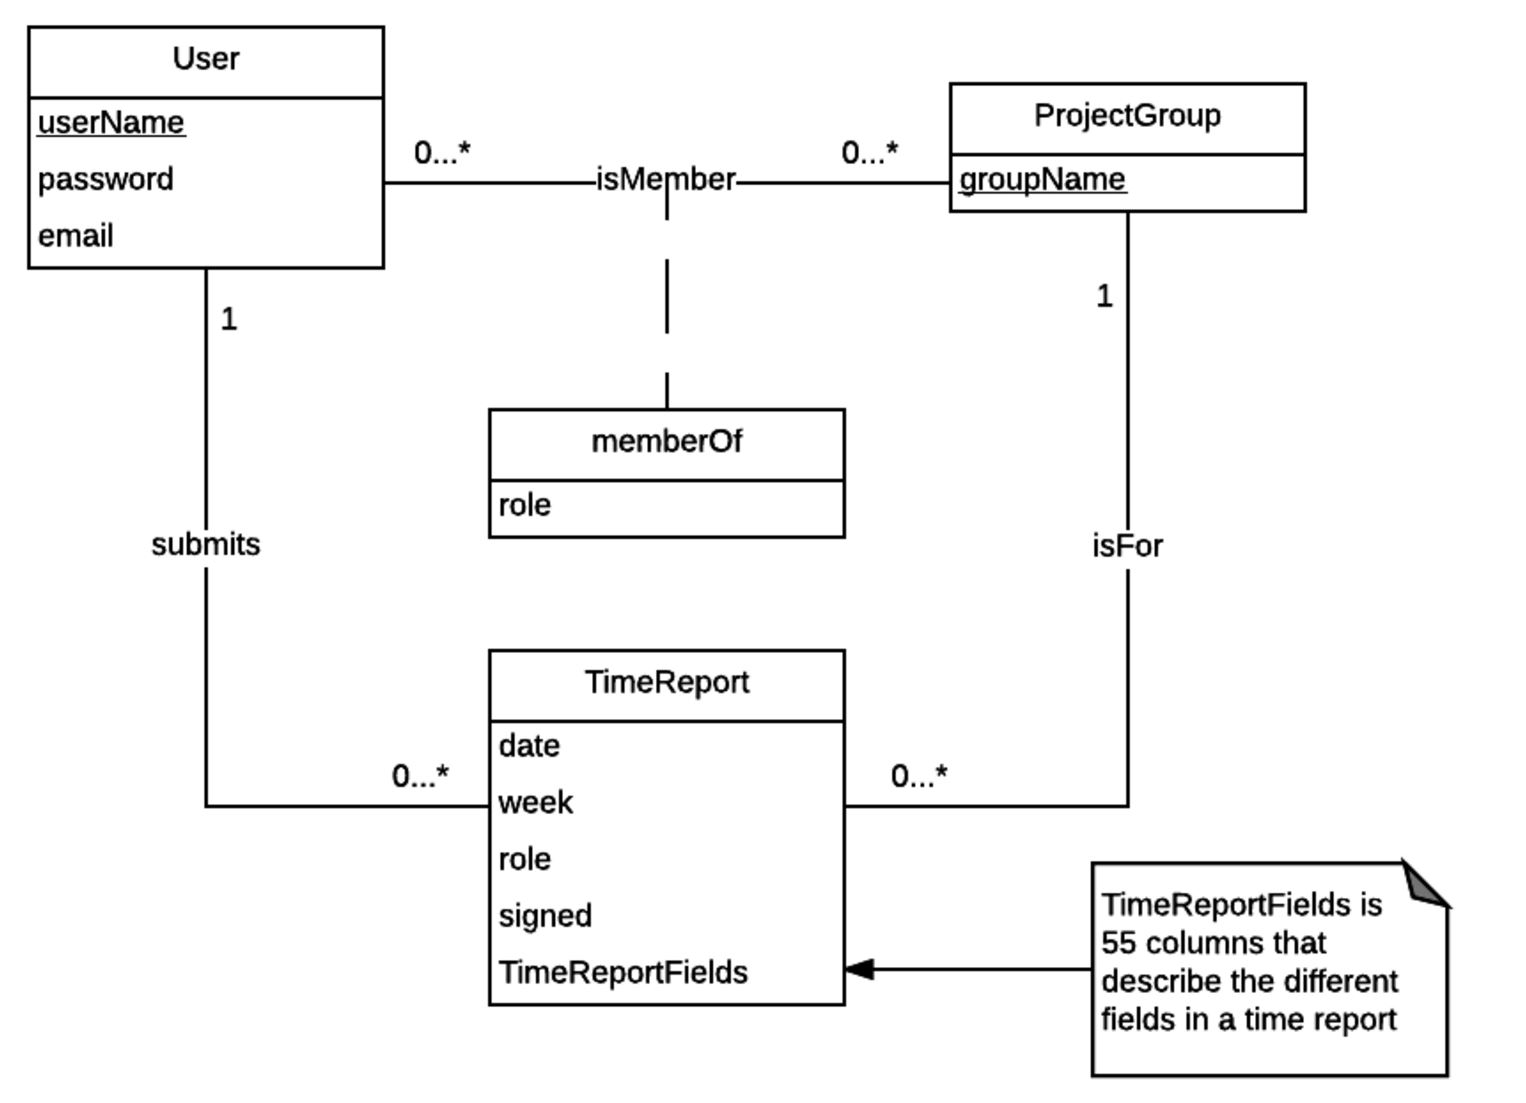
\includegraphics{ERmodel}
\end{figure}

\begin{itemize}
\item[] \textbf{Users}(\underline{userName}, password, email)
\item[] \textbf{ProjectGroups}(\underline{groupName})
\item[] \textbf{TimeReports}(``field 1'', ... , ``field 65'')
\item[] \textbf{memberOf}(\textit{groupName}, \textit{member}, role)
\end{itemize}

\newpage
\subsection{Users}
\begin{itemize}
\item[] \textbf{Users}(\underline{userName}, password, email)
\end{itemize}
\paragraph{Users} är en tabell som innehåller användare som är inlagda i systemet. Den består av tre kolumner: userName, password och email. userName är primary key vilket innebär att det endast kan finnas en användare med det användarnamnet.

\begin{figure}[H]
\centering
\caption{Tabellen har följande utseende:}
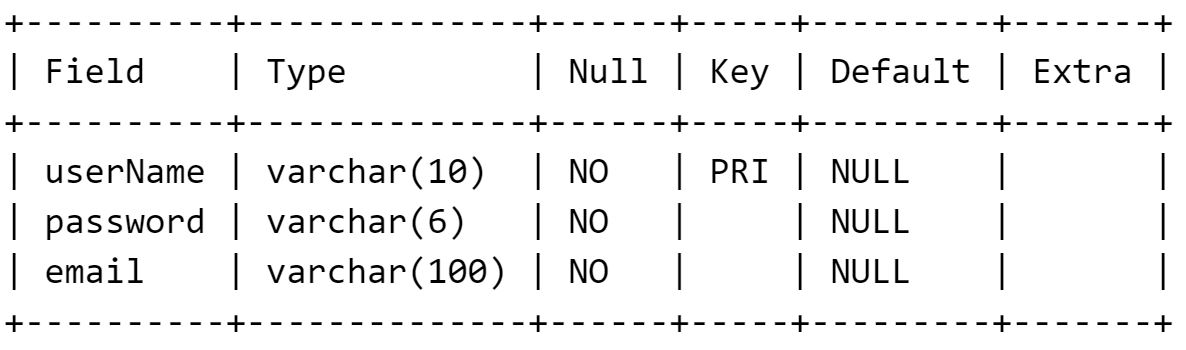
\includegraphics[width=8cm]{UsersTable}
\end{figure}

\begin{lstlisting}[frame=single, caption={Tabellen kan konstrueras med följande SQL-satser:}]
mysql> CREATE TABLE Users (
    -> userName varChar(10) NOT NULL,
    -> password varChar(6) NOT NULL,
    -> email varChar(100) NOT NULL,
    -> PRIMARY KEY (userName));
\end{lstlisting}

\subsection{ProjectGroups}
\begin{itemize}
\item[] \textbf{ProjectGroups}(\underline{groupName})
\end{itemize}
\paragraph{ProjectGroups} är en tabell som innehåller de olika projektgrupperna i systemet. Den innehåller endast en kolumn, groupName, som är satt som ``primary key'' vilket innebär att alla projektgrupper måste ha unika namn.

\begin{figure}[H]
\centering
\caption{Tabellen har följande utseende:}
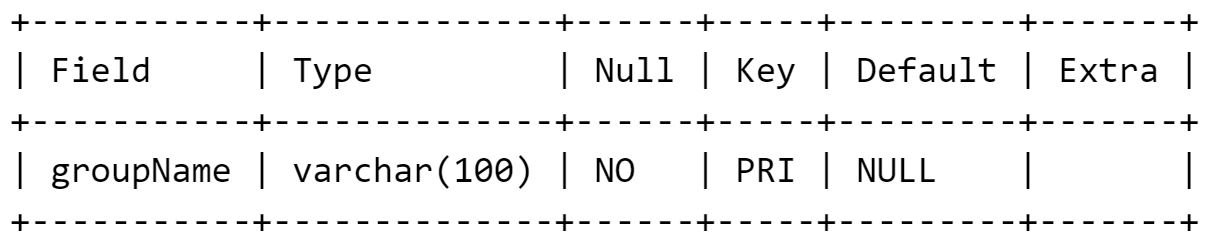
\includegraphics{ProjectGroupsTable}
\end{figure}

\begin{lstlisting}[frame=single, caption={Tabellen kan konstrueras med följande SQL-satser:}]
mysql> CREATE TABLE ProjectGroups (
    -> groupName varChar(100),
    -> PRIMARY KEY (groupName));
\end{lstlisting}

\subsection{TimeReports}
\paragraph{TimeReports} är en tabell som innehåller all information som rör tidrapporterna. Då tabellen har många kolumner (65 st) visas den inte här. För att få ut relevant information ur tidrapporterna så finns det en hjälp-procedure som tar fram relevant information för tillfällen då detta kan kräva många rader kod. För enklare fall så räcker det med en vanlig SELECT. Det finns även två triggers, en för när man lägger in en ny rad, och en när man uppdaterar en existerande rad, som väljer rätt roll för användaren, uppdaterar de totala värdena för aktiviteterna med subaktiviteter (11-19), uppdaterar den totala tiden spenderad för subaktiviteterna (d, i, f och r) och den totala tiden rapporten avser.
%%%%Finns inga SQL-satser, eller tabell antagligen för att den var för lång

\subsection{memberOf}
\begin{itemize}
\item[] \textbf{memberOf}(\textit{groupName}, \textit{member}, role)
\end{itemize}
\paragraph{memberOf} är en relationstabell som beskriver relationen mellan användare och de olika projektgrupperna. Den har tre kolumner: groupName, member och role. Kolumnerna groupName och member är tillsammans satta som UNIQE, vilket resulterar i att en medlem endast kan vara medlem i samma grupp en gång (en roll per projektgrupp). \textit{groupName} är en ``foreign key'' som refererar till \textbf{ProjectGroup(groupName)} och \textit{member} är en ``foreign key'' som refererar till \textbf{Users}(\underline{userName}).\newline

\begin{figure}[H]
\centering
\caption{Tabellen har följande utseende:}
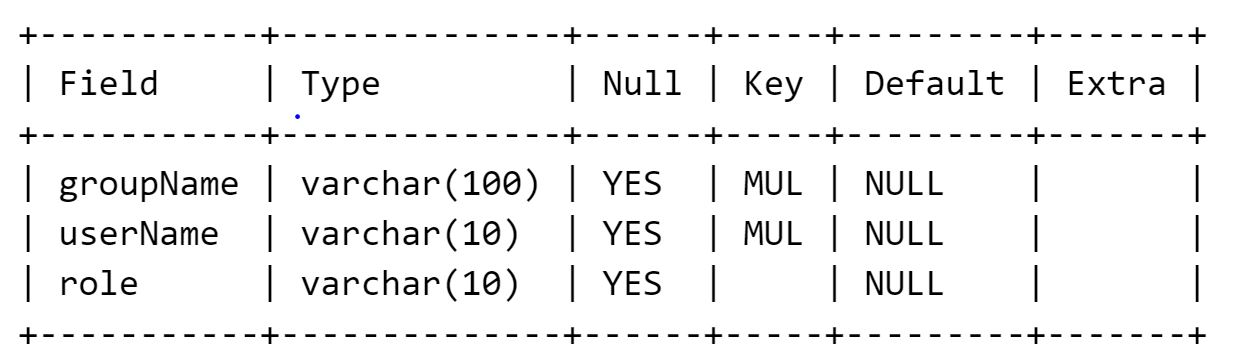
\includegraphics{memberOfTable}
\end{figure}

\begin{lstlisting}[frame=single, caption={Tabellen kan konstrueras med följande SQL-satser:}]
mysql> CREATE TABLE memberOf (
    -> groupName varChar(100),
    -> member varChar(10),
    -> role varChar(10),
    -> UNIQUE (groupName, member),
    -> FOREIGN KEY (groupName) references ProjectGroups(groupName) 
    -> ON UPDATE CASCADE ON DELETE CASCADE ,
    -> FOREIGN KEY (member) references users(userName) 
    -> ON UPDATE CASCADE ON DELETE CASCADE);
\end{lstlisting}



\section{Sekvensdiagram}
\subsection{Class LoginServlet}
\begin{figure}[H]
\centering
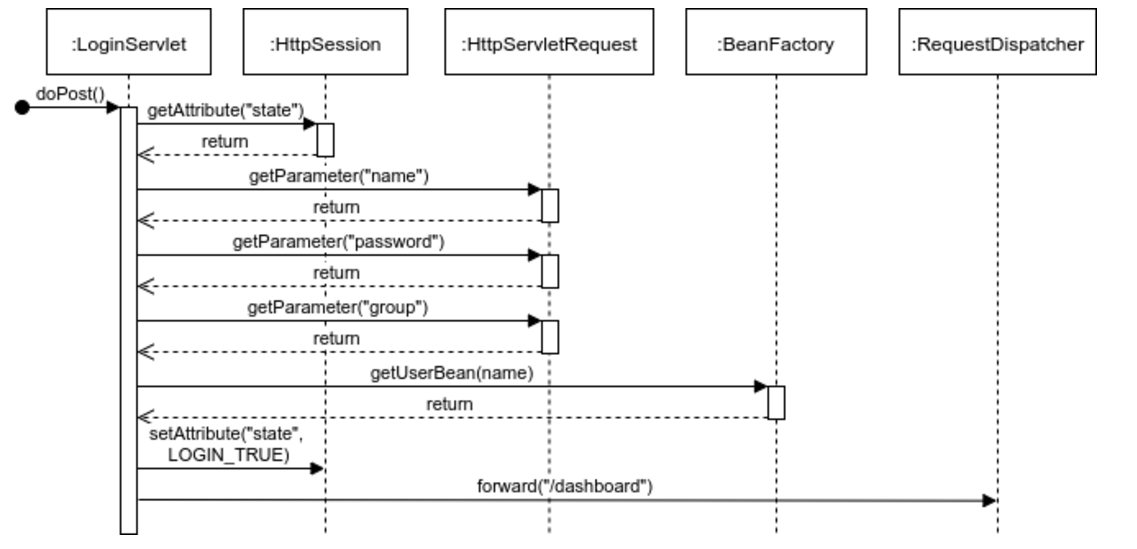
\includegraphics[width=175mm]{LoginServlet}
\caption{Sekvensdiagram som hanterar en lyckad inloggningsförfrågan}
\end{figure}

\begin{figure}[H]
\centering
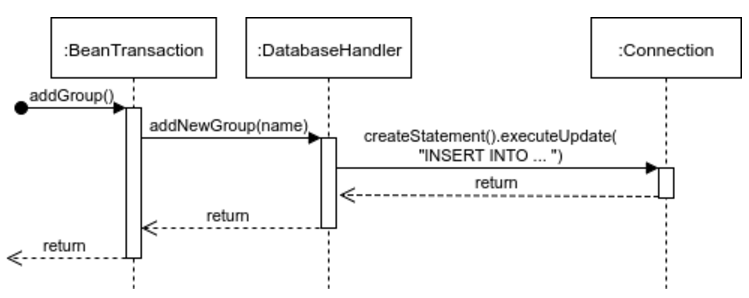
\includegraphics[width=170mm]{LoginServletFailed}
\caption{Sekvensdiagram som hanterar en icke-lyckad inloggningsförfrågan.}
\end{figure}

\subsection{Class GroupManagementServlet}

\begin{figure}[H]
\centering
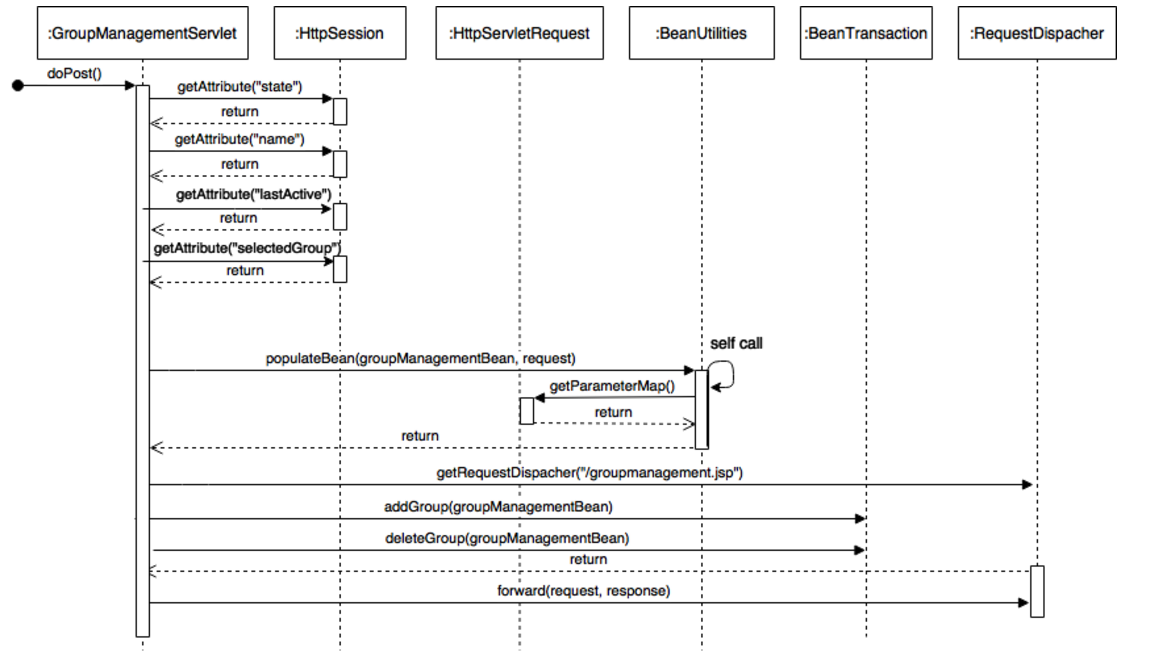
\includegraphics[width=175mm]{GroupManagementServlet}
\caption{Sekvensdiagram som hanterar tilläggande av ny användare samt borttagande av existerande användare.}
\end{figure}

\begin{figure}[H]
\centering
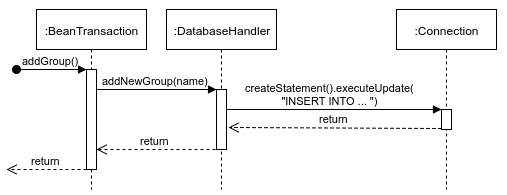
\includegraphics[width=160mm]{GroupManagementServlet2}
\caption{Sekvensdiagram som visar vad klassen BeanTransaction gör vid metoden addGroup().}
\end{figure}

\subsection{UserManagementServlet}

\begin{figure}[H]
\centering
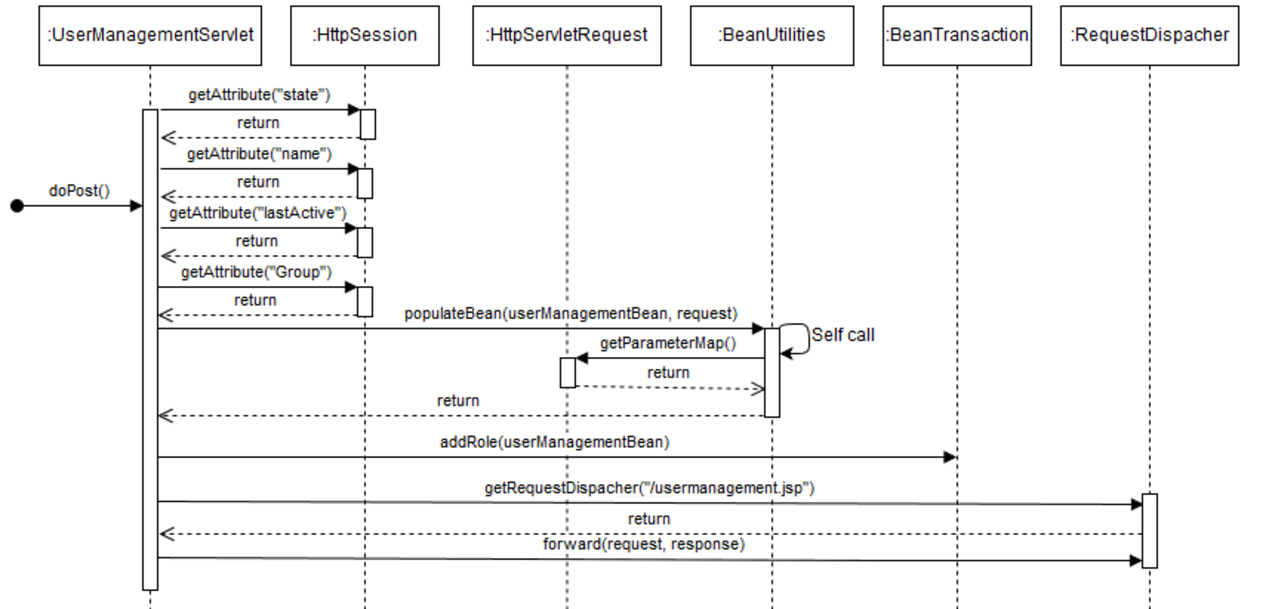
\includegraphics[width=160mm]{UserManagementServlet}
\caption{Sekvensdiagram som beskriver rolltilldelning av en projektmedlem. }
\end{figure}

\subsection{Class ReportManagementServlet}

\begin{figure}[H]
\centering
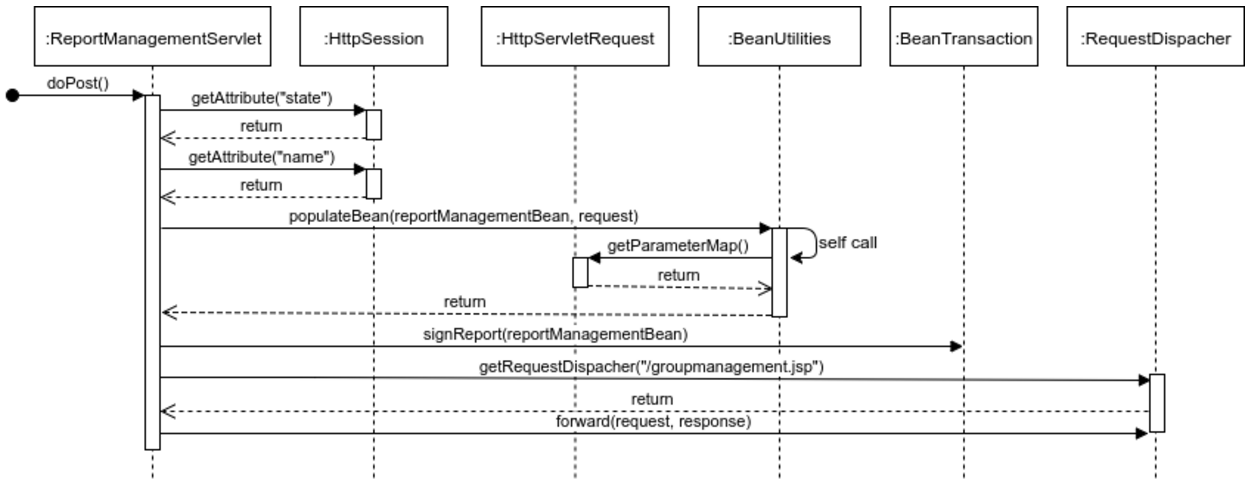
\includegraphics[width=175mm]{ReportManagementServlet}
\caption{Sekvensdiagram som beskriver hur en veckorapport signeras av en projektledare. }
\end{figure}

\begin{figure}[H]
\centering
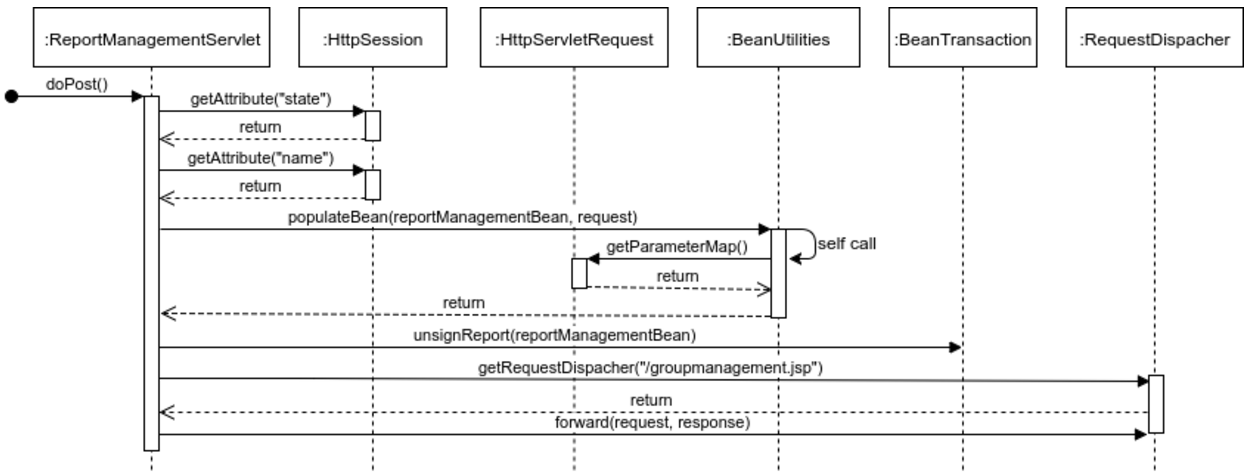
\includegraphics[width=175mm]{ReportManagementServlet2}
\caption{Sekvensdiagram som beskriver hur en eller flera veckorapporters signering tas bort av en projektledare.}
\end{figure}

\subsection{ReportServlet}

\begin{figure}[H]
\centering
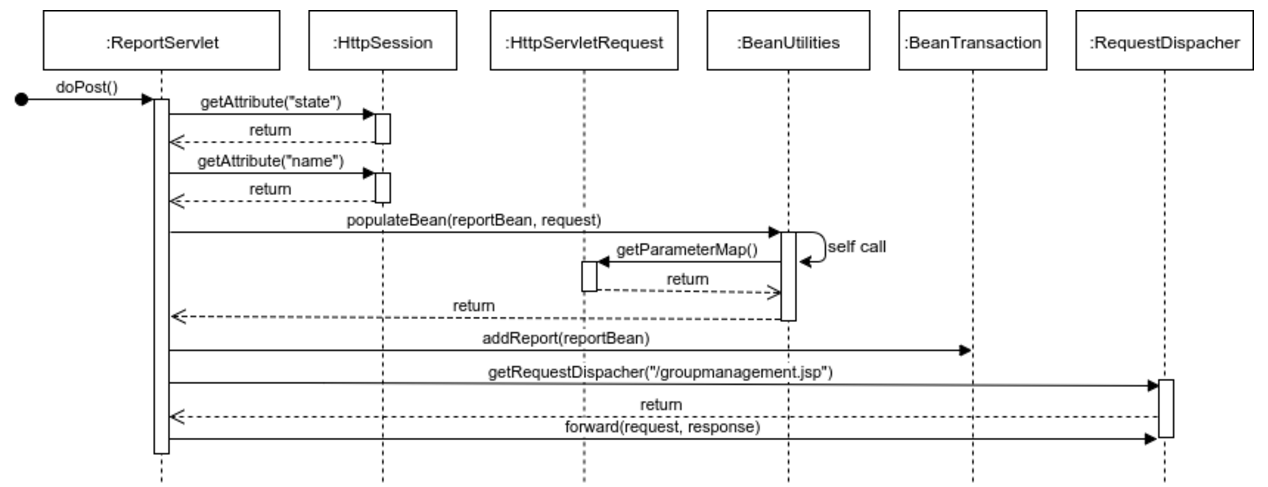
\includegraphics[width=175mm]{ReportServlet}
\caption{Sekvensdiagram som beskriver hur en projektmedlems tidrapportering sparas.}
\end{figure}

\subsection{UserServlet}

\begin{figure}[H]
\centering
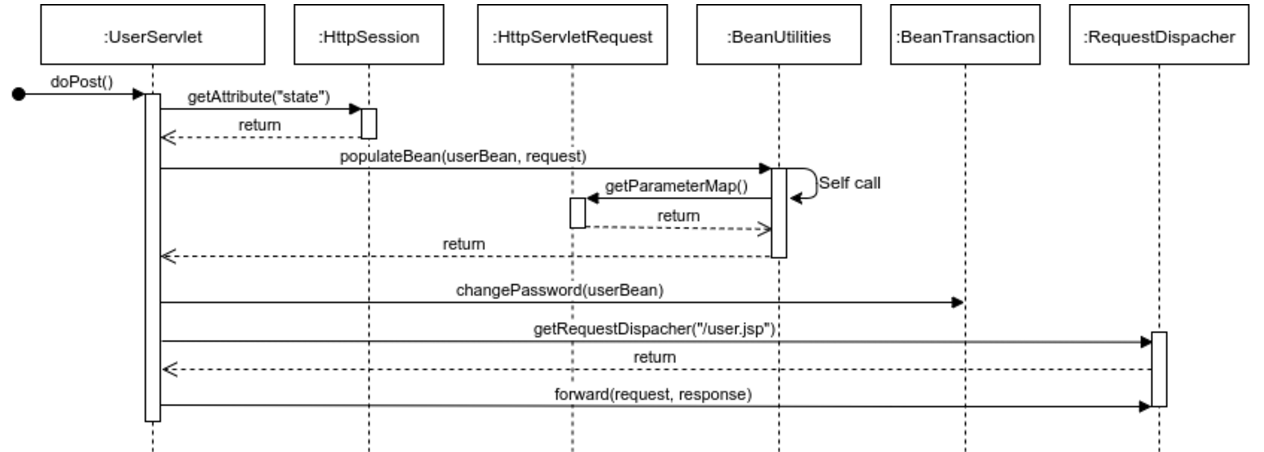
\includegraphics[width=175mm]{UserServlet}
\caption{Sekvensdiagram som beskriver en lyckad ändring av en projektmedlems lösenord.}
\end{figure}

\begin{figure}[H]
\centering
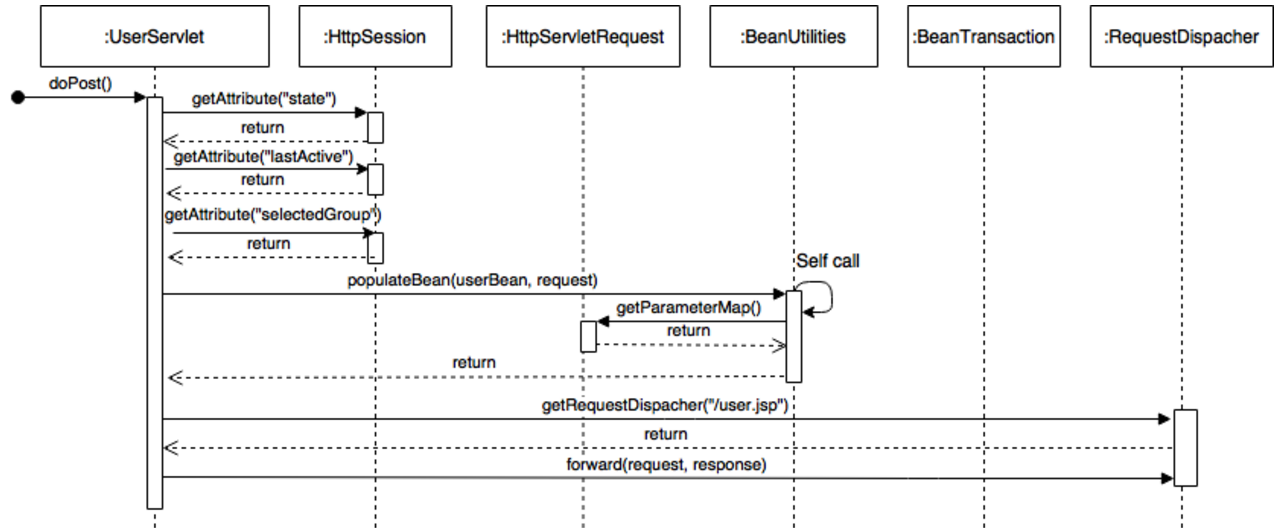
\includegraphics[width=175mm]{UserServletFailed}
\caption{Sekvensdiagram som beskriver en misslyckad ändring av en projektmedlems lösenord. }
\end{figure}

\subsection{DashBoardServlet}

\begin{figure}[H]
\centering
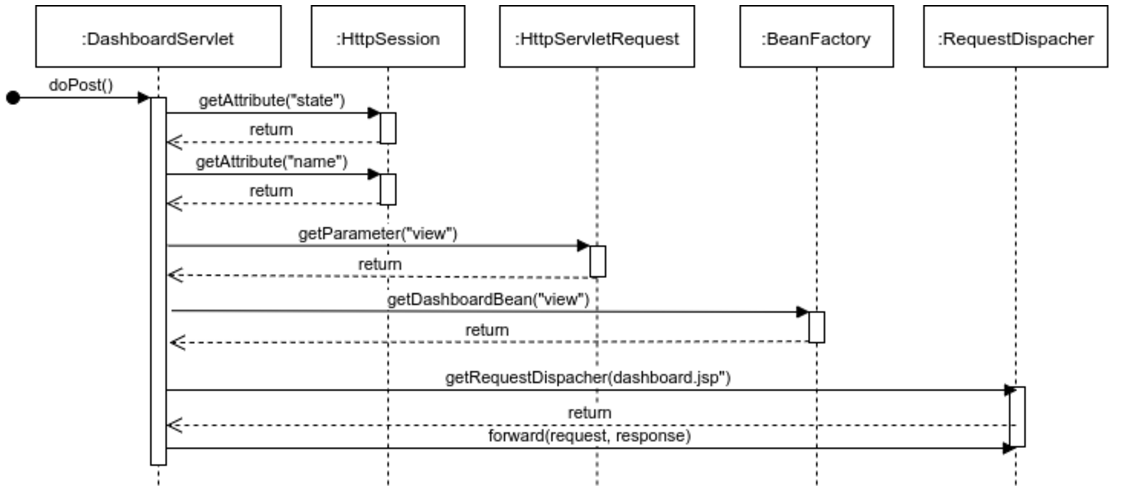
\includegraphics[width=175mm]{DashBoardServlet}
\caption{Sekvensdiagram som beskriver användandet av DashBoardServlet}
\end{figure}


\section{Routing}
Servlets konfigureras till att lyssna på specificerat HTTP URL-mönster, genom användning av @Webservlet-annotering inuti klassfilen. Denna annotering bearbetas av Tomcat vid så kallad deployment

\begin{table}[htb]
\centering
\begin{tabular}{|l|l|}
\hline
Servlet-Class           & URL-Pattern                                                     \\ \hline
LoginServlet            & \begin{tabular}[c]{@{}l@{}}./\\ ./login\\ ./logout\end{tabular} \\ \hline
GroupManagementServlet  & ./management/groups                                             \\ \hline
UserManagementServlet   & ./management/users                                              \\ \hline
ReportmanagementServlet & ./management/reports                                            \\ \hline
ReportServlet           & ./report                                                        \\ \hline
DashBoardServlet        & ./dashboard                                                     \\ \hline
UserServlet             & ./settings/user                                                 \\ \hline
\end{tabular}
\caption{Routing}
\label{my-label}
\end{table}
\FloatBarrier


\section{Appendix A}

Klassdiagrammet för Java-klasser. Diagrammet är delat på mitten, så slutstrecket i fig. A.1 fortsätter i fig. A.2.
\begin{figure}[H]
\centering
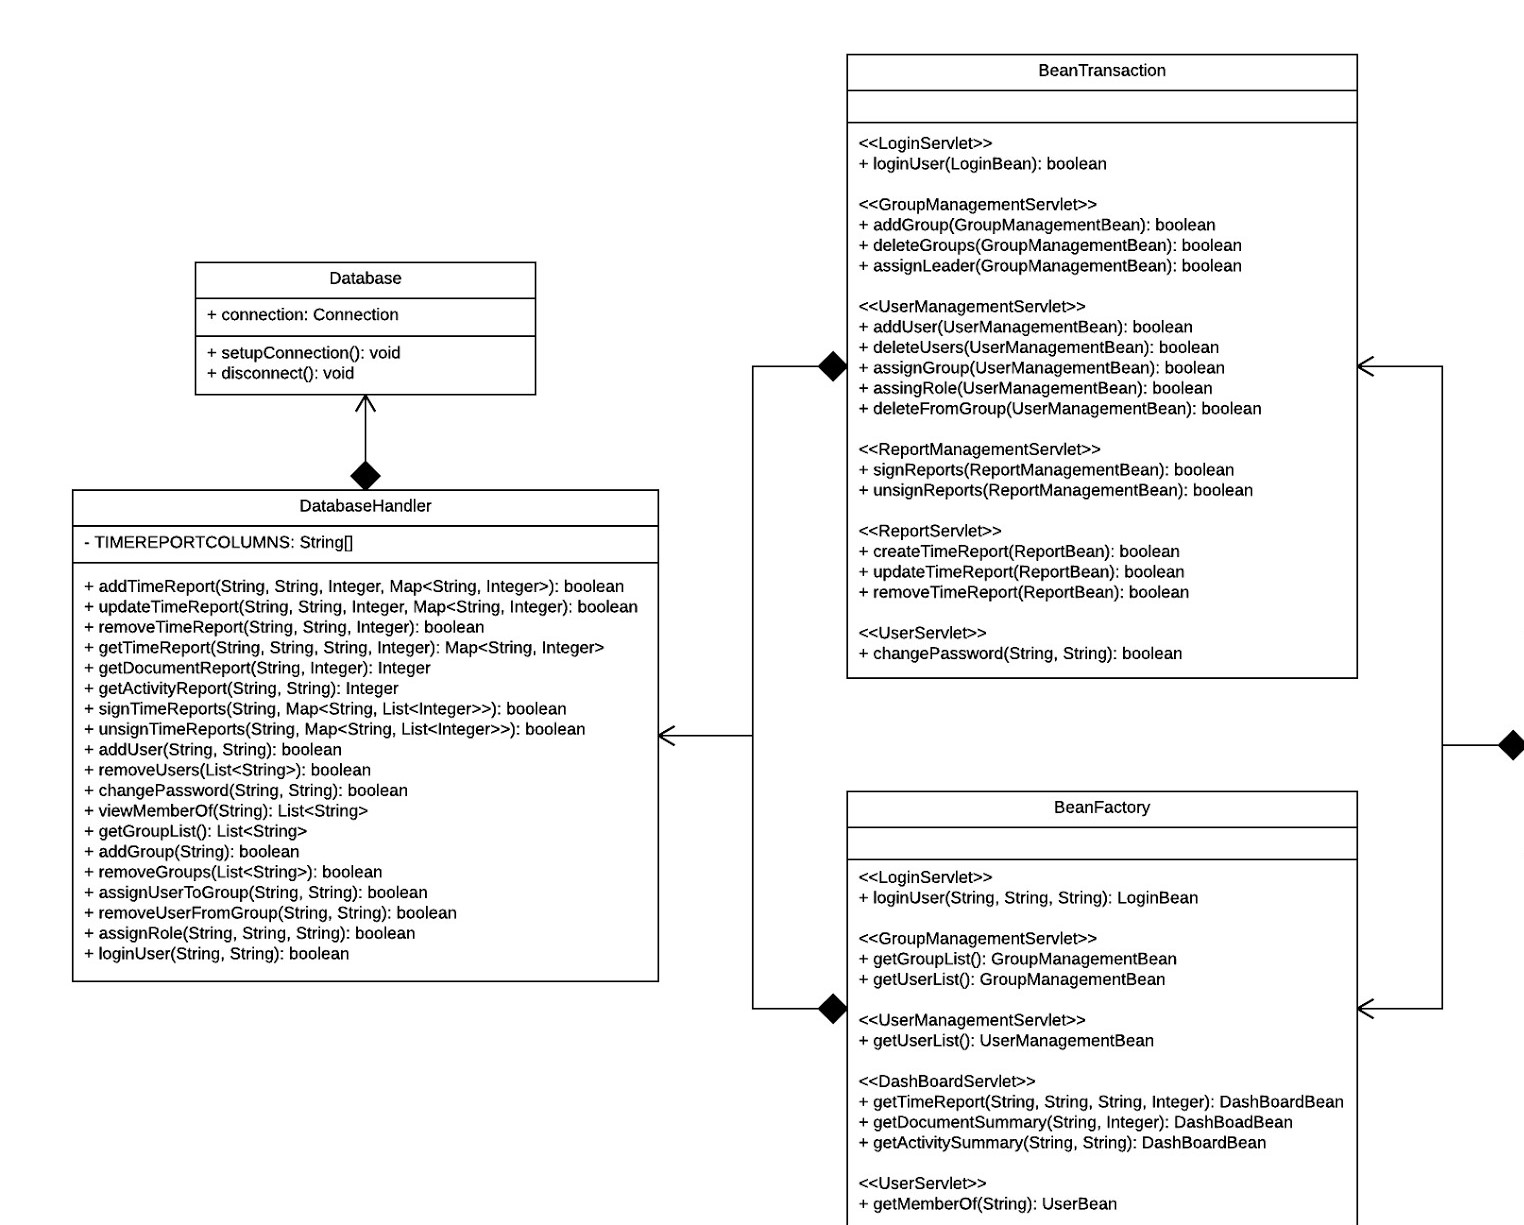
\includegraphics[width=13cm]{Klassdiagram1}
\caption{Första halvan i klassdiagrammet.}
\end{figure}
%Figur A.1. Första halvan i klassdiagrammet.
\begin{figure}[H]
\centering
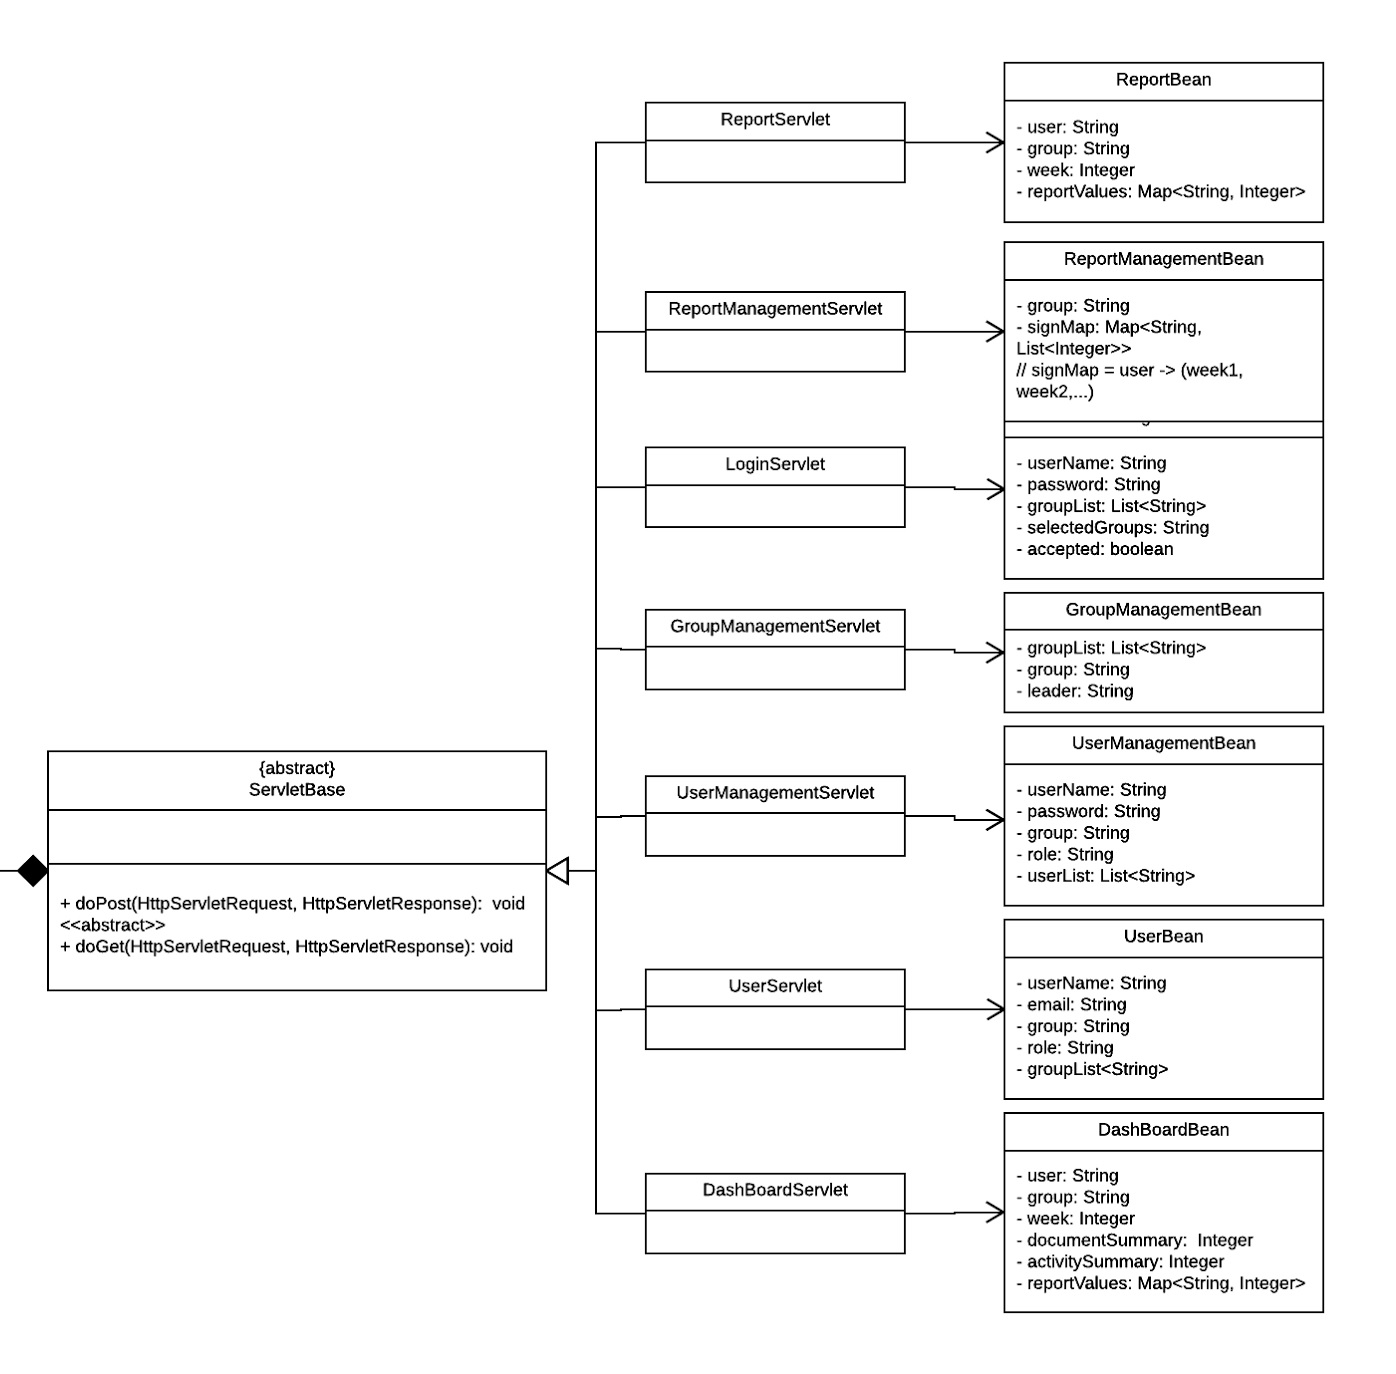
\includegraphics[width=14cm]{Klassdiagram2}%%lyckas inte få till denna bild
\caption{Andra halvan i klassdiagrammet.}
\end{figure}
%Figur A.2. Andra halvan i klassdiagrammet.


\end{document}
